\documentclass{article}
\usepackage[margin=1in]{geometry}
\usepackage{indentfirst}
\usepackage{graphicx}
\graphicspath{ {\string~/Desktop/tex/} }
\linespread{1.75}
\title{Predicting Box Office Performance for Upcoming Movies}
\author{Anudeep Gavini \and Sean Sodha \and Omar Abdul-Rahim}
\date{December 4, 2017}

\begin{document}
\maketitle

\section*{Introduction}
\vspace{0.2in}

Before a big movie hits the theaters, there are always speculations on how well the movie will perform when it comes to its actors, director, genres, etc. As movie-lovers, we wanted to see if there was a way to predict the box office performance for any kind of movie released from Hollywood. 

We are using the “TMDB 5000 Movie Dataset” from Kaggle to predict the box office performance for upcoming movies. This dataset contains two files, “movies” and “credits.” The “movies” file contains information regarding a movie’s title, genre, date, rating, budget, language, runtime, box office revenue, and other factors. The “credits” file contains information regarding the entire cast and crew in great detail and is listed in order for each movie. We have joined these two datasets and below are some graphics that give an overview of the data. 

\begin{figure}[ht]
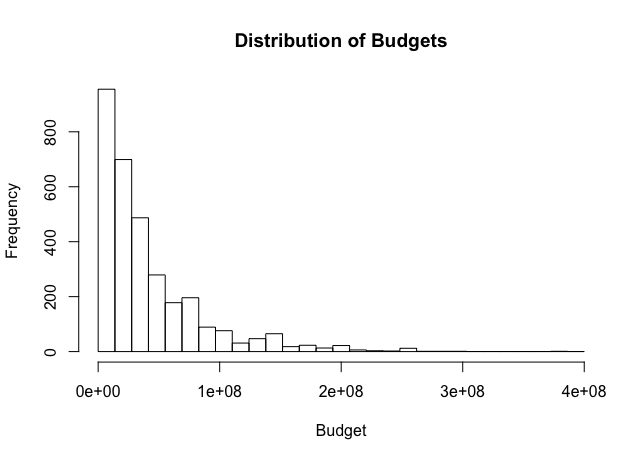
\includegraphics[width = 0.5\textwidth]{budget.png}
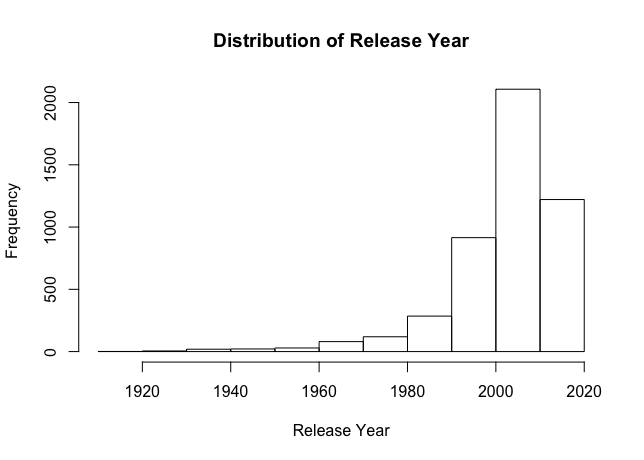
\includegraphics[width = 0.5\textwidth]{release.png}
\end{figure}

\begin{figure}[ht]
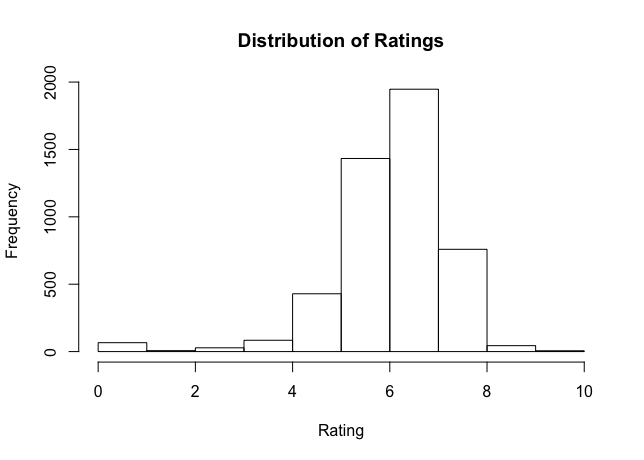
\includegraphics[width = 0.5\textwidth]{rating.png}
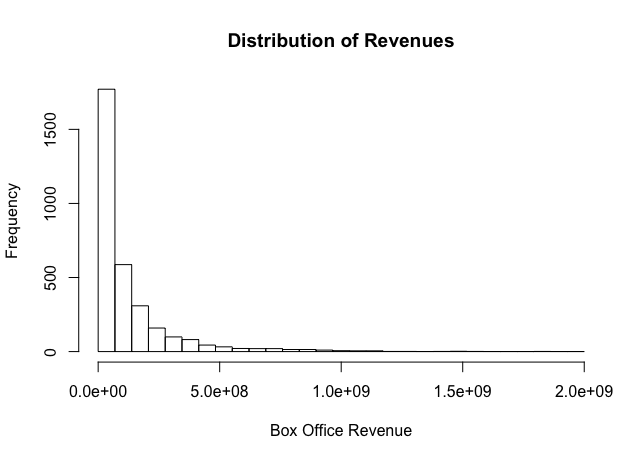
\includegraphics[width = 0.5\textwidth]{revenue.png}
\end{figure}

We certainly have an excess of information as well as incomplete portions, so we had to clean our data. As we progress through this report, we will explain the following:  
\begin{enumerate}
    \item How we cleaned our original dataset
    \item What features we chose to work with
    \item Which models we used as well as their accuracy 
\end{enumerate}

\section*{Data Cleaning}
\vspace{0.2in}

Originally, our dataset consisted of excess information such as the number of crew members, the language of the movie, etc. We cleaned up most of the data in Excel and we also noticed that several of the movies had a budget of \$0, a revenue of \$0, or some were missing both. We observed that those data points were mostly international movies and since we were focusing only on Hollywood movies, we removed them since this would not affect our data so much. After eliminating movies with a budget and revenue of \$0, we were left with 3,200 movies which is still a substantial amount of data especially when we have amazing granularity in our data. We chose the following features to help with predicting the box office for movies: Number of Total Movie Credits the Director Has, Budget, Cumulative Awards of the Top 5 Billed Actors Appearing in the Movie, Release Date, Genre Classification, and Revenue.

\section*{Handling Genres}
\vspace{0.2in}

One issue we encountered was dealing with genres. A movie's genre seems often highly correlated with its success; for example, we believe a romantic comedy will tend to have a broader appeal and therefore a higher box office performance than an indie horror film. However, this is nearly impossible to predict deterministically, given that movies often straddle multiple genres or cannot be properly described in most mainstream genre categories.

Within our data set, an example was ascribed anywhere from one to six different genres, each with a unique identifying code, in a single column. In order to make this useful, we wrote a script that parsed through the column looking for the first three listed genres for each film (we chose to use only the first three for simplicity's sake and to prevent over-fitting). If a movie had fewer than three genres listed, then the script outputted the listed genres and null cells for the remaining slots. This outputted a matrix full of binary cells with the movies on one axis and all possible genres on the other axis. If a genre-movie pair was correct, the cell held a value of 1 (otherwise, 0).

We chose this approach to handling genres because it allowed the model to decide what made a genre important. We could have arbitrarily given some genres a higher propensity to perform well at the box office, but this could make our model work under false assumptions. Instead, if a model decides that a particular genre means good box office performance, then all examples with that genre get an equal application of the weight chosen, and no other examples get the benefit of that weight.

\section*{Modifying the Release Date}
\vspace{0.2in}

We knew that the release date of a movie would most certainly affect a movie’s box office performance. In order to properly incorporate the release date, we needed to convert the release date to the number of the day in the year. For instance, the 07/04 (July 4th) date would be converted to 185.

\section*{Implementing a Web Scraper}
\vspace{0.2in}

The only information that was given in our dataset for the actors was just their name. This does not help us to determine who would be the best actor to put in a movie. Therefore, we needed a way to quantify their performance in previous movies. So we implemented a web scraper in Python. Each actor has a unique ID on IMDB, so we first wrote a web scraper to retrieve the top 10,000 actor’s names as well as their unique ID. Since, each actor has a page of awards on the IMDB website, we used the web scraper to search that page for the total number of awards won by that actor, and then plot the data in a csv file. We have appended this data to the TMDB dataset that we obtained. 

\section*{Additional Adjustments}
\vspace{0.2in}

One more thing we had to consider was inflation over time. Figures from 1950 will not be useful when compared with 2017 figures. In order to fix this, we found the inflation rate for each year and multiplied.

In addition, because of the seasonality factor of films, we wanted to give advantage to some time periods over others. In order to do this, we sorted the films into the following categories based on release date: spring, summer, back to school, Halloween, Oscars/holiday, post-awards. We felt that these changes would effectively capture the advantages that, say, a summer release has over a spring release.


\section*{Validation}
\vspace{0.2in}

In order to validate the models we used, we used 10-fold cross validation. We believed that the results from cross-validation show that our model is not severely under-fit or over-fit.

\section*{Models Implemented}
\vspace{0.2in}
We chose to go with the following 4 approaches: Log-Altered Linear Regression, Log-Altered Huber Loss Regression, Log-Altered Anova-Based Decision Tree, and Log-Altered Neural Network.

\section*{Log-Altered Linear Regression}
\vspace{0.2in}

The first model we chose to run was the simplest - a linear regression seemed like a logical starting point. However, our results were not very good. Due to the nature of our data set, the budget figure was disproportionately affecting the outcome. For reference, budget figures could be in the hundreds of millions, whereas some of our other features held values in the hundreds or even binary values. So, we decided the best way forward was to take the natural log of the budget and revenue columns. The results were much better. Below is a figure showing our linear regression with the log adjustment applied:

\begin{figure}[ht]
\centering
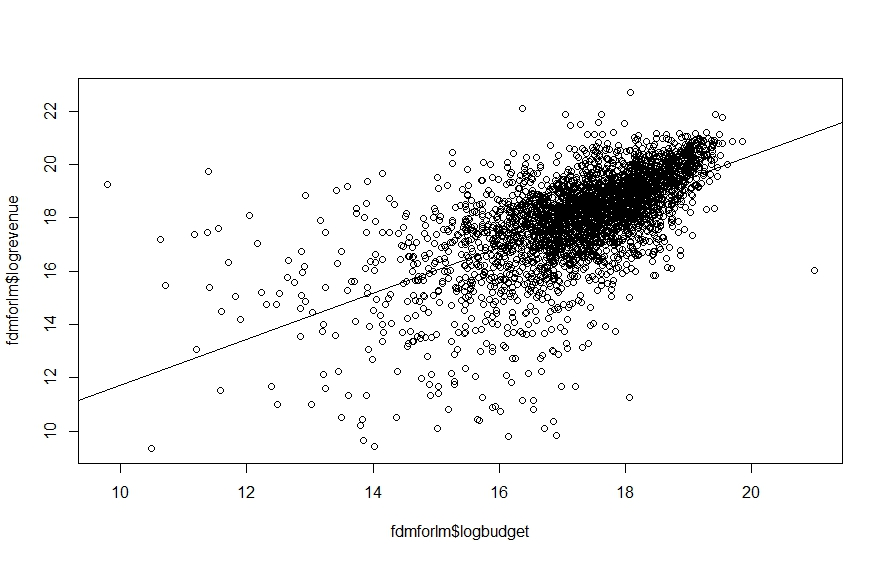
\includegraphics[width = 0.6\textwidth]{logbudgvlogrev}
\end{figure}

Visually, the data does look somewhat linear. To give a sense for the distribution of outcomes, we have included a histogram of our predicted values:

\begin{figure}[ht]
\centering
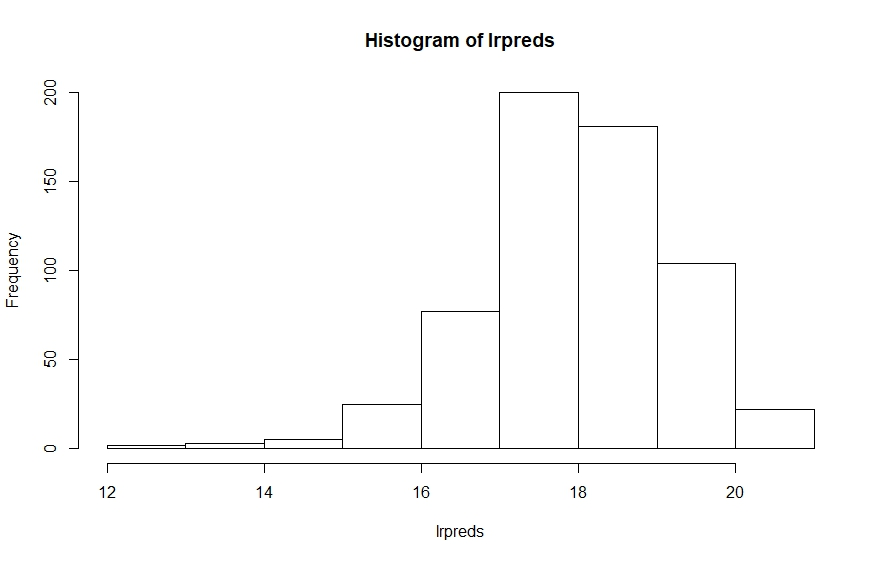
\includegraphics[width = 0.6\textwidth]{histpred}
\end{figure}


Our call command for the model was the following:

\begin{equation}
lm(formula = logrevenue ~ genre1 + genre2 + genre3 + release + logbudget + runtime + credits + awards, data = train)
\end{equation}

This model had an R$^2$ value of 0.4437. Based on this model, the most significant features impacting a film's revenue were: it being a summer release (release), its budget size (logbudget), how long it is (runtime), the pedigree of its director (credits), the number of awards it has received (awards) and its genre (genre1, genre2, and genre3). The genres that were most positively impactful were: Family, Adventure, Animation.The genres that were most negatively impactful (meaning that these genres connoted poor performance) were: Foreign, Western, War. An interesting finding here is that movies with generally positive messages tended to do better than movies with more somber or aggressive messages.

\section*{Log-Altered Huber Loss Regression}
\vspace{0.2in}

The second model we chose to run was a Huber Loss Regression model, which seemed like the logical next step from a simpler linear regression model.  Once again, we chose to use the log of the budget and revenues to smooth out the disproportionate effect these two variables had on the data.  Also specifically for this model, we had to exclude the genres from the formula.  Thus, our input formula for this model was actually:

\begin{equation}
lm(formula = logrevenue ~ release + logbudget + runtime + credits + awards, data = train)
\end{equation}

This was due to both technical limitations of the package being used to perform this function.  The package required that the input and response sets were of the same type, and thus we were forced to remove categorical variables from this formula. 


After testing the trained model on the test split of our data, we got $R^2$ values of $.3514$, and Root Mean Squared Errors of $1.52122$.  We can also compare the distributions of the true and predicted logs of the revenues:

\begin{figure}[ht]
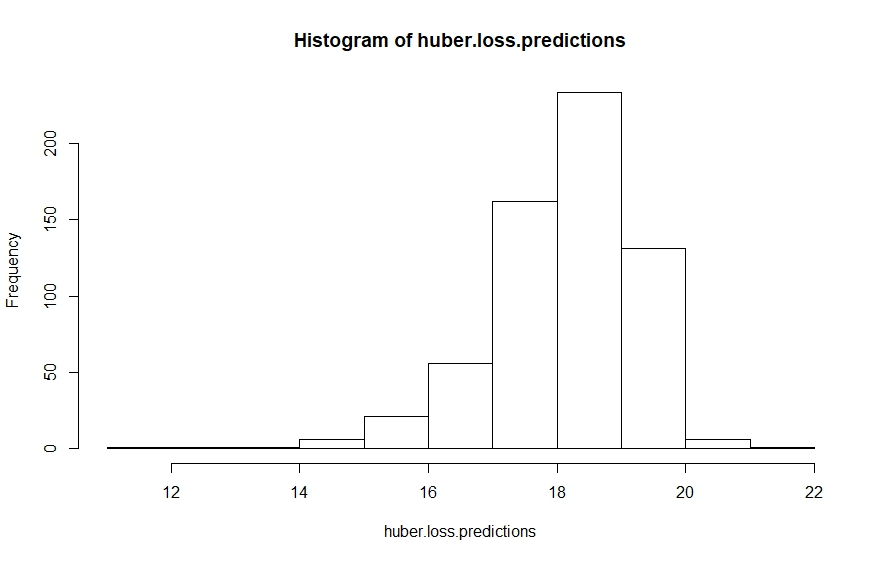
\includegraphics[width = 0.5\textwidth]{hlp.jpeg}
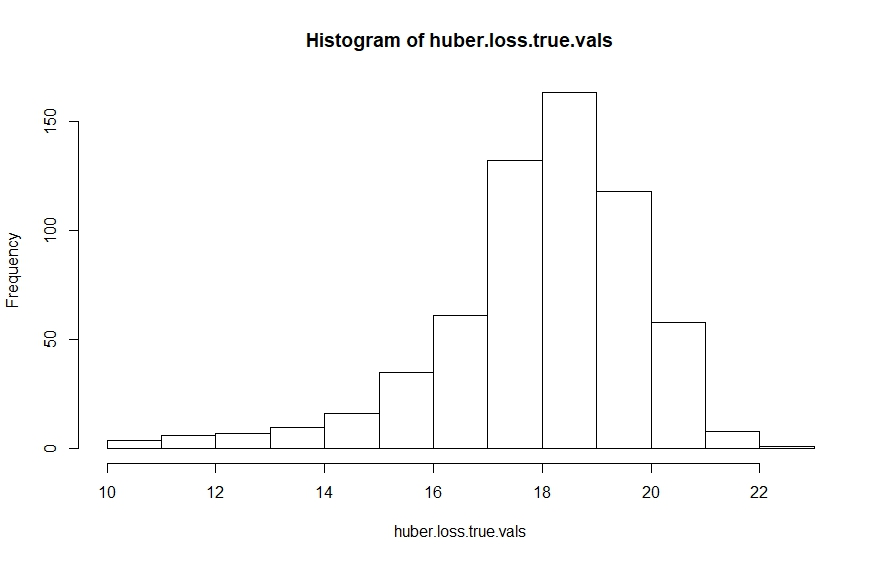
\includegraphics[width = 0.5\textwidth]{hltv.jpeg}
\end{figure}


\section*{Log-Altered Anova-Based Decision Tree}
\vspace{0.2in}

For the next model, we chose to use an Anova-Based Decison Tree to create a regression model.  We chose the Anova function, as most other approaches to the decision tree focus on classification, which we felt would not be appropriate given that revenue is a continuous variable.  We continued  to use the log of the budget and revenues in this model as well. We also switched back to our original formula for this and the following model.

After testing the trained model on the test splits of our data, we got $R^2$ values of $.380512$, and Root Mean Squared Errors of $1.3978$.  We can also compare the distributions of the true and predicted logs of the revenues:

\begin{figure}[h]
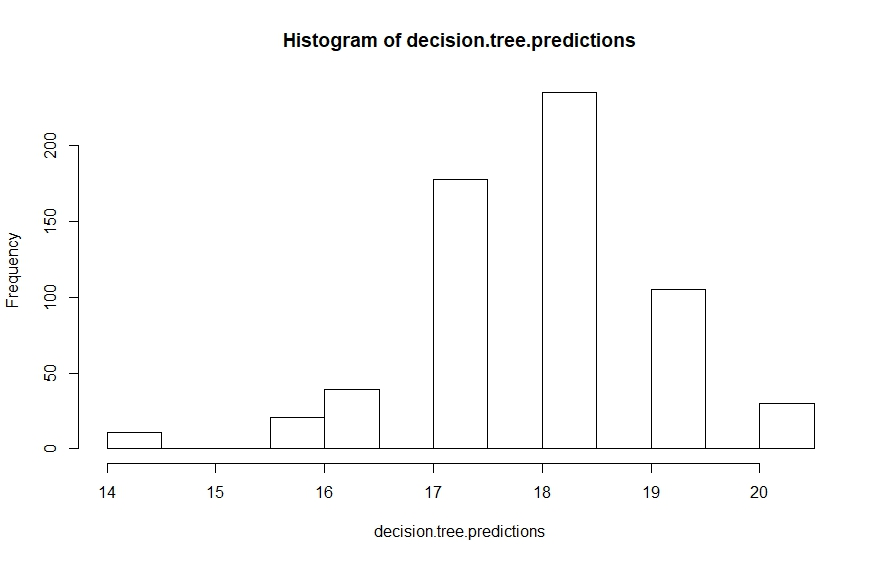
\includegraphics[width = 0.5\textwidth]{dtp.jpeg}
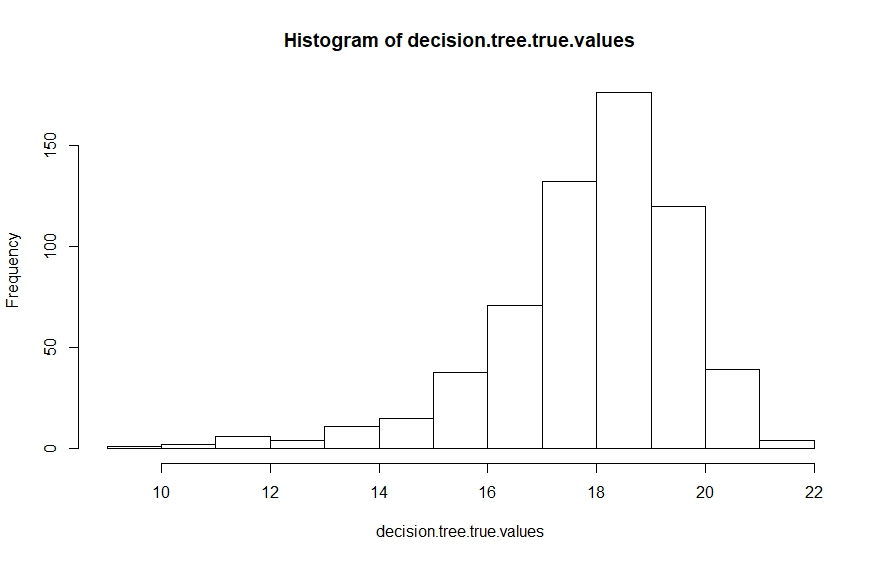
\includegraphics[width = 0.5\textwidth]{dttv.jpeg}
\end{figure}

\section*{Log-Altered Neural Network}
\vspace{0.2in}

For the next model, we chose to create a single-layer neural network using the elmNN package in R. We used the same regression formula as above.  We estimated that we would have about 70 input nodes - one for each numerical column in our training data, 20 for each genre in the genre1 column, 20 for each genre in the genre2 column, 20 for each genre in the genre3 column, and 6 for each season in the release column.  Thus, we chose to use 30 nodes in the hidden layer, and proceeded to train the neural network on the testing data.

After testing the trained model on the test splits of our data, we got $R^2$ values of $.103358$, and Root Mean Squared Errors of $1.764$.  We can also compare the distributions of the true and predicted logs of the revenues:

\begin{figure}[ht]
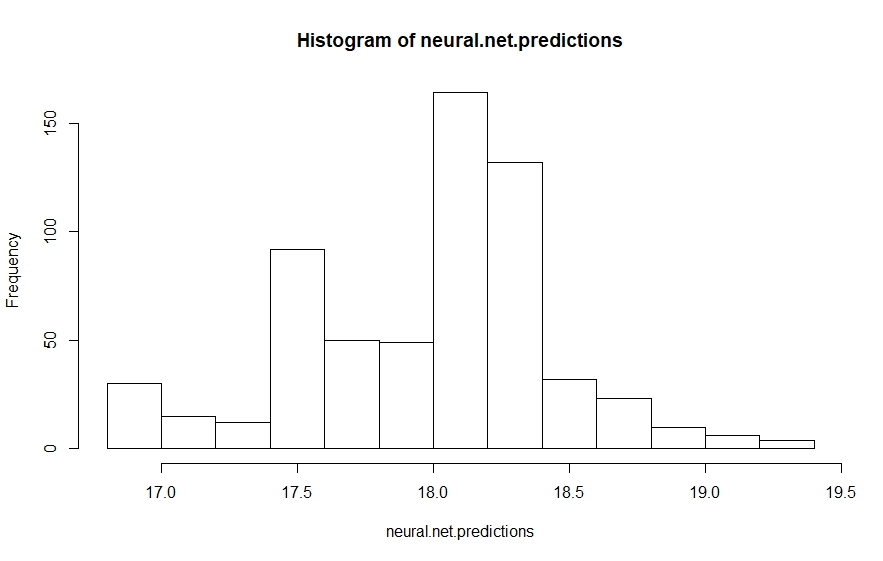
\includegraphics[width = 0.5\textwidth]{nnp.jpeg}
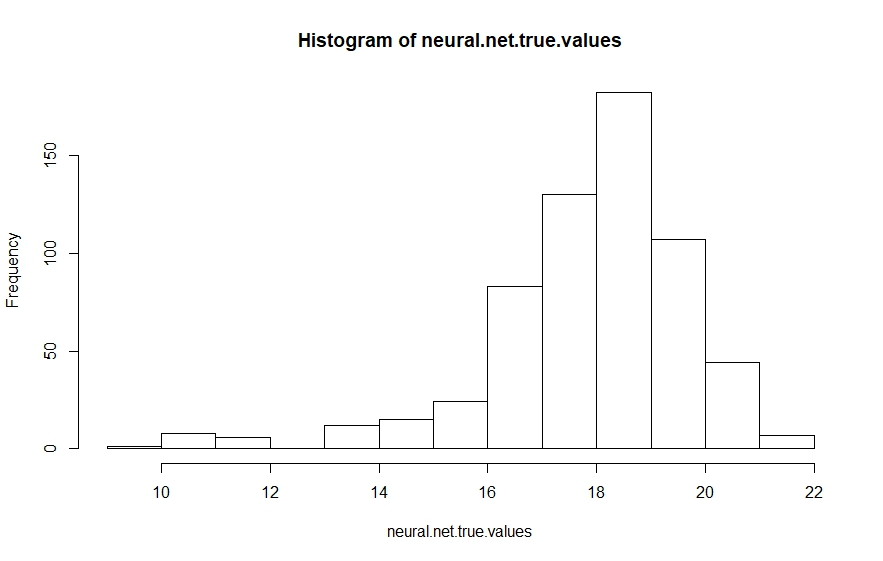
\includegraphics[width = 0.5\textwidth]{nntv.jpeg}
\end{figure}

This result was actually a bit surprising, as it turned out the neural net ended up constraining the revenue results to a far smaller range than the true values.  We expected this to be more accurate, but it was not the case

\section*{Conclusion}
\vspace{0.2in}


In sum, the model that performed the best for us was the linear regression. It had the highest R$^2$ value, which generally means lowest prediction error. Because of the model’s simplicity, we feel confident in saying that the model was not over-fit to the training data, so that should not factor into our evaluation.

One interesting finding was that low budget movies almost always have low revenues, but high budget movies are not easy to predict. It was difficult to create a very good model based off of what was supposed to be our most reliable predictor. More sophisticated models might have run into issues dealing with this disparity and run a bit wild. This might explain why the linear regression, our most simplistic model, ended up performing the best.

While much work was done to find novel ways to predict box office performance, we find it difficult to guarantee our models as surefire predictors for industry professionals. However, considering the difficult human factor, this tool proves to be a relatively useful predictor of risk. In other words, if a producer is making a film with certain preliminary attributes, this tool might be able to tell how good a chance their film has of doing generally well. We hope to learn more about the nuances of this industry that may lend us modeling insight in the future.
\end{document}